\section{Durchführung}
\label{sec:Durchführung}

Bei dem Versuch wird eine Messapparatur entsprechend Abbildung 4 verwendet. 
\begin{figure}
    \centering
    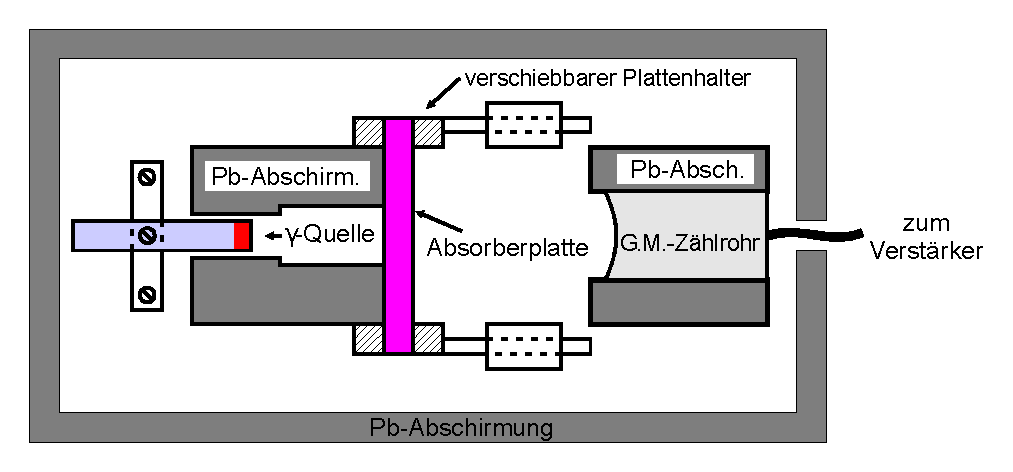
\includegraphics[width=\linewidth]{pictures/messaparatur.pdf}
    \caption{Aufbau der verwendeten Messapparatur für die $\gamma$-Strahlung. \cite{v704}}
    \label{fig:messaparatur}
\end{figure}

Die Strahlungsquelle kann darin in einer Haltung befestigt werden kann. 
In einem gewissen Abstand befindet sich ein Plattenhalter, in dem die Platten unterschiedlicher Dicke eingespannt werden. 
Dahinter befindet sich ein Geiger-Müller-Zählrohr, mit dem die Intensität der Strahlung gemessen werden kann. 
Dieser gesamte Aufbau ist wiederum von einer Bleiabschirmung umgeben, 
um die Strahlung nach außen hin abzufangen beziehungsweise um die Apparatur vor äußeren Einflüssen zu schützen.
Ein ähnlicher Aufbau mit Aluminium statt Blei wird für die $\beta$-Strahlung verwendet.

Zu Beginn des Versuchs wird eine Nullmessung für $\qty{900}{\second}$ durchgeführt, um die Hintergrundstrahlung zu messen.
Danach wird eine $\gamma$-Strahlungsquelle eingebaut, hier $\ce{^{137}Cs}$,
und für 10 Platten verschiedener Dicken von je Eisen und Kupfer nacheinander eingesetzt.
Bei jeder Platte wird je nach Dicke in einem passenden Zeitintervall von $100$ bis $\qty{500}{\second}$ die Aktivität gezählt.

Analog wird dies für eine $\beta^-$-Strahlungsquelle, hier $\ce{^{99}Tc}$, für Aluminium wiederholt.
Auch hier ist je nach Absorberdicke auf ein passendes Zeitintervall zu achten, 
sodass der relativ statistische Fehler minimiert wird.